\documentclass{article}

\usepackage[italian]{babel}
\usepackage[utf8]{inputenc}


\usepackage{listings} % for coding like part

\usepackage{graphicx}
\graphicspath{ {./images/} }

\usepackage{hyperref} % lasciare per ultimo




 

\begin{document}
\begin{titlepage}
    \begin{center}
        \Huge{Progetto Basi di Dati}\\
        [20mm]
        \Large{Paolo Addis}\\
        \Large{Samuele Poz}\\
        \Large{Tristano Munini}\\
        [20mm]
        \Large{RENDERE CARINO}
    \end{center}
\end{titlepage}

\tableofcontents
\thispagestyle{empty}
\cleardoublepage
\setcounter{page}{1}

% REGOLE DI STILE
% - scrivere in modo impersonale no "abbiamo deciso di"
% - 


% TODO
% - abbellire hyperlinks
% - modifiche su full_er_model_02
% - rimuovere CARTELLA-CLINICA dallo schema ER della Progettazione ER
% - CARTELLA-CLINICA in DIAGNOSI-EFFETTUATA o altro


% TODO -- SCHEMI 
% - primo schema: pazinete fuori regione, attributi composti multivalore, no cartella clinica 
% - secondo schema: togli ternaria, toglie specializzazione, togli attributi composti, multivalore 
% - terzo schema: per prestazioni aggiungiamo diagnosi effettuate 

% COSE DA RICORDARE
% NEI REQUISITI
% - aggiungere numero di accessi effettuati e numero di Pazienti, Ricovero, ecc
% - Evidenziare la necessità dell'ospedale di accedere spesso alle diagnosi di un dato paziente
% NELLA FASE LOGICA
% - verrà aggiunta relazione tra PAZIENTE DIAGNOSI (es DIAGNOSI EFFETTUATE) per verificare la differenza di prestazioni
% - l'unica ridondanza è data da DIAGNOSI EFFETTUATE, la ricorsione DIAGNOSI->DIAGNOSI (o ISTANZA DI TERAPIA -> DIAGNOSI) NON è ridondanza (esprime informazioni differenti)



\section{Progettazione Concettuale}\label{sec:prog_conc}

\subsection{Raccolta ed Analisi dei Requisiti}

Si vuole modellare il seguente insieme di informazioni riguardanti un sistema per la gestione delle diagnosi e delle terapie dei pazienti ricoverati in un dato ospedale.
\begin{itemize}
  \item Di ogni ricovero, il sistema deve memorizzare il codice univoco, il nome della divisione ospedaliera (Cardiologia, Reumatologia, Ortopedia, \dots ), il paziente ricoverato, le date di inizio e fine del ricovero e il motivo principale del ricovero.
  \item Di ogni paziente, il sistema deve memorizzare il codice sanitario (univoco), il cognome, il nome, la data di nascita, il luogo di nascita e la provincia di residenza.
    Per i pazienti residenti fuori regione, vengono memorizzati anche il nome della ULSS e la regione di appartenenza.
  \item Inoltre di ogni paziente si vuole memorizzare la cartella clinica, caratterizzata dall'insieme di tutte le diagnosi del paziente.
  \item Di ogni diagnosi effettuata durante il ricovero del paziente, sono memorizzati la patologia diagnosticata, col suo codice ICD10 (classificazione internazionale delle patologie) e l’indicazione della sua gravità (grave: si/no), la data e il nome e cognome del medico che ha effettuato la diagnosi.
  \item Nella base di dati si tiene traccia delle terapie prescritte ai pazienti durante il ricovero.
    Di ogni terapia, si memorizzano il farmaco prescritto, la dose giornaliera, le date di inizio e di fine della prescrizione, la modalità di somministrazione ed il medico che ha prescritto la terapia.
    % TODO manca parte in cui si dice che la terapia è un concetto astratto
  \item Di ogni farmaco sono memorizzati il nome commerciale (univoco), l’azienda produttrice, il nome e la quantità dei principi attivi contenuti e la dose giornaliera raccomandata.
  \item Si tiene, infine, traccia delle diagnosi che hanno motivato le terapie.
    In particolare, ogni terapia è prescritta al fine di curare una o più patologie diagnosticate.
    Può capitare anche che una nuova patologia (registrata come nuova diagnosi) sia causata, come effetto collaterale, da una terapia precedentemente prescritta.
    Tale legame causa-effetto va registrato nella base di dati.
\end{itemize}
Tramite un portale web dovrà essere possibile accedere a tale base di dati ed aggiungere o rimuovere pazienti, ricoveri, diagnosi con relative terapie e farmaci. 




\clearpage
\subsection{Progettazione del Modello E-R}
%TODO
%\begin{itemize}
%  \item Descrizione procedimento Inside-Out con schemi parziali (fasi della costruzione) e descrizione testuale delle relazioni e entità
%    \begin{itemize}
%      \item Unione in attributo composto e multivalore dei principi attivi 
%    \end{itemize}
%\end{itemize}
Inizialmente abbiamo concentrato la nostra attenzione sulle entità PAZIENTE e RICOVERO perché ci sembravano fondamentali: si può dire che in assenza di un'entità che rappresenti i pazienti, l'intera base di dati perderebbe significato.
Infatti per ogni ricovero o diagnosi deve essere possibile risalire al soggetto che è stato ricoverato o a cui è stata effettuato una diagnosi, altrimenti non si potrebbe utilizzare correttamente le informazioni raccolte in passato.
RICOVERO, invece, segna i momenti in cui il paziente raggiunge e lascia la struttura ospedaliera, inoltre permette di indicare in modo univoco le visite e le cure alle quali è stato sottoposto durante questo periodo.
Abbiamo unito le due entità con una relazione chiamata VIENE-RICOVERATO che intuitivamente collega una entità PAZIENTE a molte entità RICOVERO.
Abbiamo poi costruito la tripletta FARMACO, SOMMINISTRATO-DURANTE e TERAPIA composta rispettivamente da: un'entità che rappresenta il farmaco con i relativi attributi; una relazione che permette di indicare che farmaco viene usato durante una terapia; ed infine un'entità che raccoglie i dettagli della terapia, ad esempio la dose giornaliera di farmaco da assumere.
L'entità DIAGNOSI e le rimanenti relazioni, in particolare CAUSA-EFFETTO, verranno analizzate successivamente.


\begin{figure} % TODO abbellire
  \centering
  \includegraphics[width=\linewidth]{full_er_model_01}
  \caption{Lo schema Entità-Relazioni completo}
  % TODO modificare immagine
  % - Specializzazione con Paziente Fuori Regione
  % - Diagnosi come entità debole con chiave (Effettuata Durante, Data)
  % - Rimuovere medico da Terapia
  \label{figure_ER_01}
\end{figure}

\subsubsection{Le Entità} % TODO sarebbe meglio creare subsubsubsection o paragrafi per ogni entità?
\begin{itemize}
\item PAZIENTE: dai requisiti si capisce chiaramente che bisogna tener traccia di \textit{codice sanitario}, \textit{cognome}, \textit{nome}, \textit{data di nascita}, \textit{luogo di nascita} e \textit{provincia di residenza} del paziente.
    Abbiamo creato un attributo per ciascuna di queste voci e selezionato il codice fiscale come chiave primaria.
    È stata una scelta naturale perché dal testo sappiamo che il codice fiscale (d'ora in poi detto anche CF) è univoco, proprietà fondamentale per definire la chiave primaria di un'entità\footnote{Ricordiamo la definizione di chiave primaria univoca e sottoinsieme minimo TODO}.
    Per salvare gli attributi esclusivi per i pazienti fuori regione riguardanti il nome della ULSS e la regione di appartenenza, è stata creata l'entità PAZIENTE-FUORI-REGIONE, specializzazione dell'entità precedente.
    Poiché solo una frazione dell'insieme dei pazienti sarà di questo tipo la specializzazione è parziale e senza sovrapposizione(TODO si diceva così?), essendo l'unica.
  \item RICOVERO: anche in questo caso abbiamo deciso di aggiungere all'entità un attributo per ogni voce del testo, fatta eccezione per \textit{paziente ricoverato}.
    Infatti non solo sarebbe inutile ma addirittura pericoloso ripetere un'informazione che verrà modellata dalla relazione VIENE-RICOVERATO, di cui parleremo successivamente.
    Nell'immagine \ref{figure_ER_01} si può osservare l'insieme degli attributi 
  \item TERAPIA
  \item FARMACO
  \item DIAGNOSI
\end{itemize}

\subsubsection{Le Relazioni}
\begin{itemize}
  \item VIENE-RICOVERATO
  \item SOMMINISTRATO-DURANTE
  \item EFFETTUATA-DURANTE
  \item CARTELLA-CLINICA
\end{itemize}
Abbiamo prestato particolare attenzione a CAUSA-EFFETTO.
Questa relazione potrebbe sembrare eccessiva essendo sia ternaria che ricorsiva, in realtà modella molto bene un requisito fondamentale: \textit{``Può capitare anche che una nuova patologia (registrata come nuova diagnosi) sia causata, come effetto collaterale, da una terapia precedentemente prescritta.''}
Da un altro requisito sappiamo che una DIAGNOSI può essere in relazione con una TERAPIA in quanto la terapia viene prescritta solo se esiste una diagnosi che la motivi.





%\begin{figure}[h] % TODO abbellire
%\caption{Entità PAZIENTE con specializzazione e, a destra, RICOVERO}
%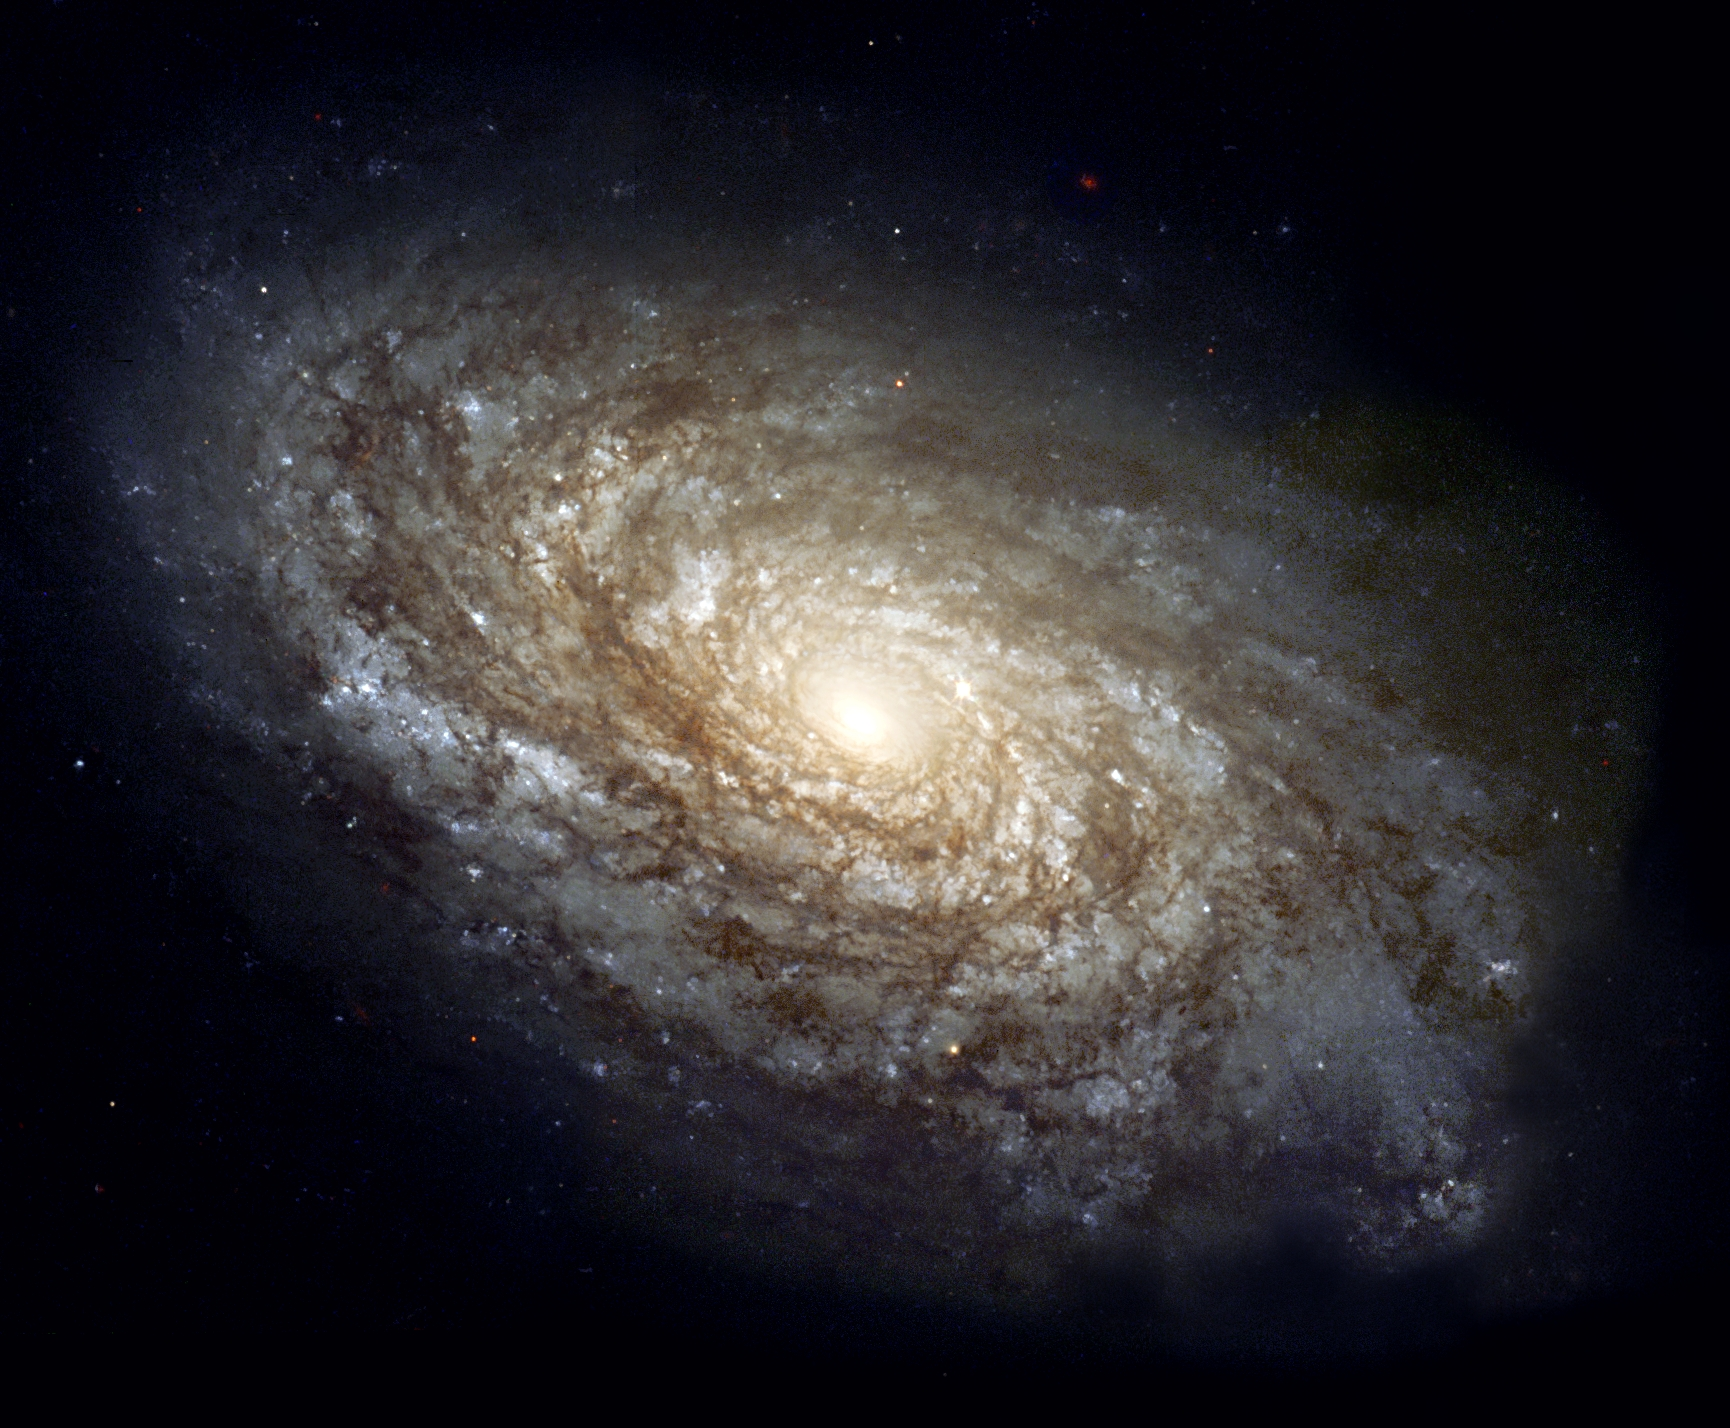
\includegraphics[width=0.4\textwidth]{galaxy}
%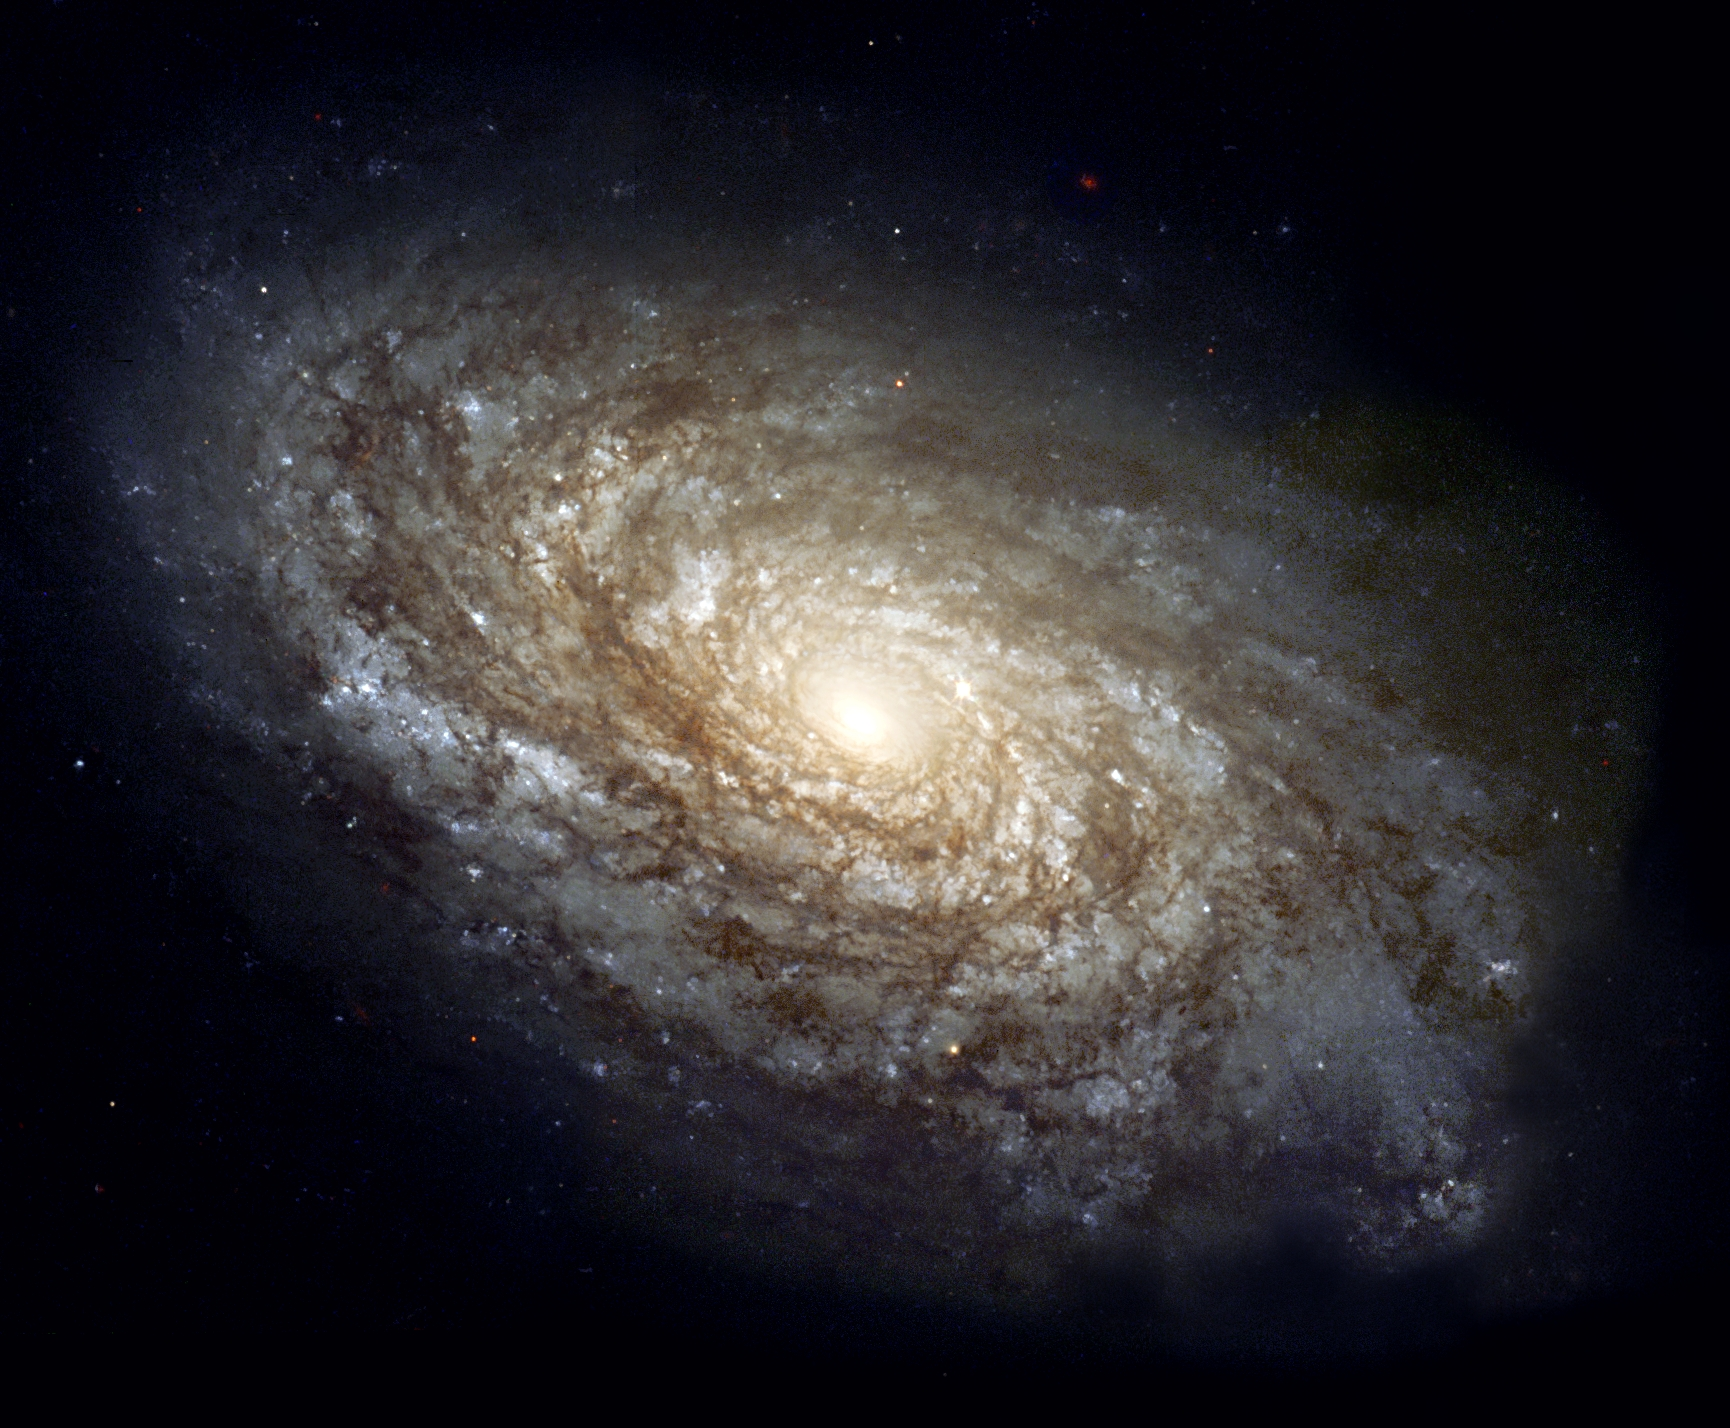
\includegraphics[width=0.4\textwidth]{galaxy}
%\end{figure}




\clearpage
\section{Progettazione Logica}
TODO
\begin{itemize}
  \item Semplificazione dei concetti
    \begin{itemize}
      \item Rimozione della relazione ternaria (vedi schema "causa effetto")
    \end{itemize}
  \item Analisi delle ridondanze (vedi fogli "cartella clinica")
  \item Rimozione delle Generalizzazioni (non presente)

  \item Partizione/merging di entità
    \begin{itemize}
      \item Eliminazione dell'attributo composto "patologia" in DIAGNOSI
      \item Partizionamento dei principi attivi in una nuova entità
      \item Cose che si potrebbero aggiungere:
        \begin{itemize}
          \item Partizionamento entità inteso come separazione degli attributi in base alle operazioni (almeno le principali)
          \item Partizionamento di una relazione (si può fare con MEDICO collegato a PAZIENTE e DIAGNOSI) ???????
            (secondo Tri 'fare solo se non abbiamo abbastanza materiale')
        \end{itemize}
    \end{itemize}
  \item Selezione delle chiavi
    \begin{itemize}
      \item Aggiungere un codice come chiave della diagnosi (da giustificare)
    \end{itemize}
\end{itemize}
TODO guardare i commenti in file sorgente
\subsection{Ristrutturazione del Modello E-R}
\subsection{Traduzione del Modello Logico}

%% sotto un copia-incolla da vecchio file %%

% SCRIVIAMO LA LISTA DELLE TABELLE CON TUTTE LE CHIAVI BELLE DENTRO 
% SOTTO SCRIVIAMO LA LISTA: "LA RELAZIONE X è GARANTITA DA QUESTA COMBO 
%                            DI CHIAVI (Y,Z)..."
% 
% - Traduzione di VIENE-RICOVERATO (da scrivere bene perchè è la prima)
% 
% PAZIENTE (_CF_, NOME,...)
% RICOVERO (_CODICE-RICOVERO_,...,DIVISIONE-OSPEDALIERA, CF, MOTIVO)
%           . CF chiave esterna not null, 
%           . MOTIVO not null
% . Specificare che la traduzione cattura la partecipazione (0,N)(1,1)
%   e non (1,N)(1,1), bisogna introdurre un vincolo esterno per garantire
%   (1,N)
% 
% - Traduzione di EFFETTUATA-DURANTE 
%   . lo creiamo aggiungendo una chiave esterna su DIAGNOSI con not null
% 
% - Traduzione di CARTELLA-CLINICA
%   . lo creiamo aggiungendo una chiave esterna su DIAGNOSI con not null
% 
% - Traduzione di SOMMINISTRATO-DURANTE
%   . lo creiamo aggiungendo una chiave esterna su TERAPIA con not null
% 
% - Traduzione di CURATA-DA e di ISTANZA-DI e EFFETTO-COLLATERALE
%   . ISTANZA-DI-TERAPIA (__DIAGNOSI_,_TERAPIA__,...,DIAGNOSI-EC) 
%   DIAGNOSI e TERAPIA e DIAGNOSI-EC sono chiavi esterne.
%   La coppia DIAGNOSI e TERAPIA è chiave. 
%   Si deve inserire UNIQUE per DIAGNOSI e non per la coppia per 
%   garantire (1,1).      
%   Si deve inserire un vincolo esterno per garantire (1,N) su terapia
%   Si deve inserire UNIQUE su DIAGNOSI-EC per garantire 1 tra DIAG e EC




\clearpage
\section{Progettazione Fisica}
\subsection{Nuovi Indici}




\clearpage
\section{Definizione della Base di Dati in SQL}
\subsection{Definizione delle Tabelle}
\subsection{Popolamento della Base di Dati}
\subsection{Definizione di Query Significative}




\clearpage
\section{Analisi Dati in R}




\clearpage
\section{Portale Web}
\subsection{Interfaccia Grafica}
\subsection{Comunicare con pgAdmin}



\end{document}

\cleardoublepage
% Code example
\begin{lstlisting}[language=bash,title={bash version}]
#!/bin/bash
echo "Hello , world!"
\end{lstlisting}
